\subsubsection{\textit{GitHub}}


Já o \textit{GitHub} é uma plataforma de hospedagem de códigos que utiliza o \textit{Git} como controle de versão. O \textit{GitHub} possui uma grande interação com repositórios \textit{Git}, concentrando uma grande comunidade de desenvolvedores que colaboram para milhões de projetos \cite{CHACON2014}.

\begin{figure}[h]
	\caption{\label{fig_github}Repositório do projeto hospedado no \textit{GitHub}.}
	\begin{center}
		\resizebox{1\linewidth}{!}{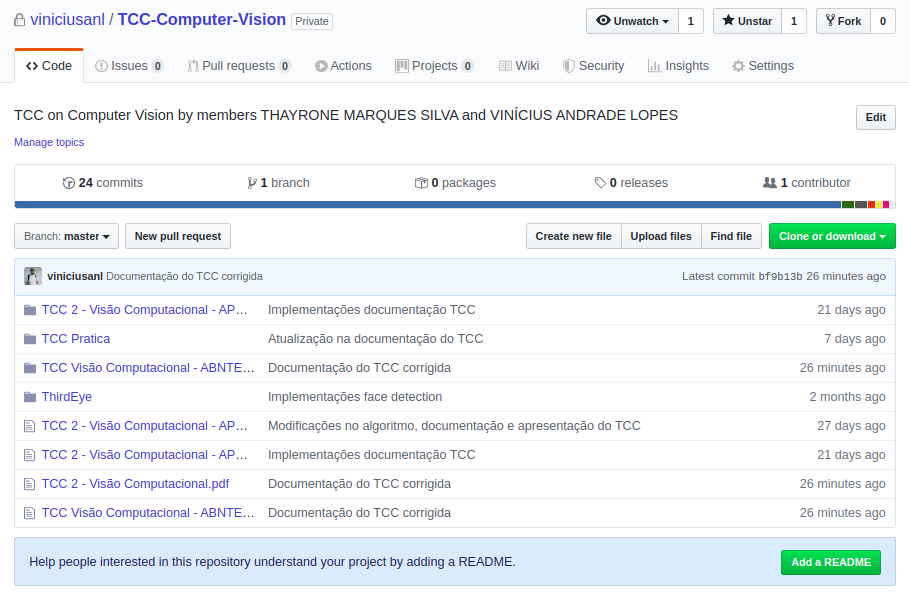
\includegraphics{4-Conteudo-Bibliografico/4-Ferramentas-de-Desenvolvimento-do-Projeto/github.png}}
	\end{center}
	\centering \legend{Fonte: Elaborada pelos autores.}
\end{figure}

A \autoref{fig_github} mostra o repositório utilizado para hospedar todos os arquivos relacionados a este projeto.

Ainda segundo \citeonline{CHACON2014}, o \textit{GitHub} hospeda a maior porcentagem de repositórios \textit{Git}. Isso ocorre porque a plataforma também disponibiliza recursos de gerenciamento de código, como por exemplo o rastreamento de problemas, revisão de código, edição \textit{online} do código, dentre outros.